\documentclass[a4paper,12pt]{article}
\usepackage{caption}
\usepackage{subcaption}
\usepackage{float}
\usepackage[T1]{fontenc}
\usepackage[italian]{babel}
\usepackage[utf8]{inputenc}
\input funzioni.sty
\input funzioni2.sty
\floatstyle{ruled}
\usepackage{hyperref}
\usepackage{graphicx}
\usepackage{amsmath}
\usepackage{amssymb}
\usepackage[width=125mm]{caption}
\usepackage{tikz}
\usepackage{amsthm}
\usepackage{algorithm2e}
% Dimensione della pagina
\setlength{\oddsidemargin}{.3in}  % Distance from the left edge -1 inch 
\setlength{\textwidth}{145mm}     % Normal width of the text
\setlength{\topmargin}{.25in}     % Distance from top to PAGE'S HEAD -1 inch
\setlength{\textheight}{225mm}    % Height of the body of page
\setlength{\headheight}{0mm}      % Height of a box containing the head
\setlength{\parskip}{0.5mm}		  % Extra vertical space before a paragraph
\setlength{\parindent}{9mm}       % Width of the indentation 
\linespread{1.12}                 % Line spacing        
\renewcommand{\floatpagefraction}{.9}

\begin{document}
\author{Stefano Mandelli\\
Matricola: 861838}
\title{\bf \Huge Confronto delle prestazioni CPU-GPU per la simulazione di un reticolo di Ising-2D}
\date{13 - Luglio - 2016}
\maketitle
\section*{Introduzione}
In questo lavoro vengono messe a confronto le prestazioni di CPU\footnote{Central Processing unit} e GPU\footnote{Graphics Processing Unit}, usando come banco di prova un modello fisico ben conosciuto di cui sono note, in modo analitico, le espressioni delle varie grandezze fisiche che si vogliono simulare. Il modello in questione \`e il \emph{reticolo di Ising bidimensionale}. 

Durante l'implementazione da CPU a GPU, \`e stato possibile riportare il codice, da un ambienete all'altro, mantenendo lo stesso algoritmo e quindi lo stesso numero di operazioni che vengono fatte durante l'aggiornamento dei siti reticolari.

\`E stato possibile riportare da un ambiete all'altro anche il generatore di numeri pseudorandom, in modo da rendere consistente la valutazione dello speed-up. Se si fosse usato un generatore di numeri pseudorandom diverso, la comparazione sarebbe stata correlata anche al tipo di implementazione del \emph{Generatore di Numeri Pseudorandom (PNRG)}. 

Il lavoro consiste in una prima presentazione del modello fisico usato a cui seguir\`a la presentazione dell'algoritmo usato per l'update dei siti reticolari. Una volta presentati modello e algoritmo di update viene descritta l'implementazione su GPU discutendo in primis la consistenza fisica della simulazione e successivamente i vari accorgimenti per ottimizzare le prestazioni.


\section{Scelta del modello}
Il modello di \emph{Ising-2D} è un modello che si presta molto bene ad essere parallelizzato in quanto è un tipico modello interagente a corto range. Per questo tipo di interazioni \`e facile trovare strategie di parallelizzazione efficaci.

Il modello di Ising è caratterizzato da un reticolo in $D$ dimensioni. Ad ogni cella del reticolo viene associato uno spin che può essere solo del tipo $s_i=\lbrace +1, -1 \rbrace$ a seconda che la direzione del dipolo magnetico, associato alla cella $i-esima$ del reticolo, risulti verso l'alto o verso il basso. 

Il sistema è descritto dall’Hamiltoniana di Ising
\newl{\mathcal{H}=-J\sum_{\langle i,j\rangle}s_is_j -h\sum_{i}s_i,}
dove $h$ identifica un eventuale campo magnetico uniforme esterno. La prima sommatoria è  su tutte le coppie di siti primi vicini e $J$ indica la costante di accoppiamento tra spin. 

In questo lavoro si considera il caso il caso $D = 2$ dimensionale, $J > 0$ e a campo magnetico esterno nullo quindi $h = 0$. Al limite termodinamico, il modello di Ising (escluso il caso $1D$) presenta una \emph{transizione di fase} in prossimità di una temperatura critica $T_c$ . Per temperature maggiori di $T_c$ il sistema \`e perfettamente \emph{paramagnetico}. Per temperature inferiori invece si ha un fenomeno di \emph{magnetizzazione spontanea}. 

Le principali grandezze fisiche che possono essere calcolate sono la \emph{magnetizzazione media} del sistema $\langle M\rangle$  e la \emph{capacità termica} a volume costante $\langle C_V \rangle$ che viene calcolata col teorema di fluttuazione-dissipazione. Tutte queste quantit\`a estensive divergono al limite termodinamico. 

Nelle simulazioni statistiche vengono considerati dei modelli finiti di $N = L \times L$ spins che si desidera confrontare per diversi size. \`E utile pertanto confrontare la \emph{densità di calore specifico} $c_V = CV /N$ e di \emph{magnetizzazione} che è la variabile coniugata al campo esterno $h$
\newl{m=\frac{1}{N}\left\langle\sum_is_i\right\rangle.}

Per il caso $h = 0$ e $T > T_c$ , $\langle M \rangle$ si annulla. Questo comportamento può essere spiegato a causa del fatto che per $T > T_c$ le fluttuazioni termiche prevalgono sulla tendenza del termine di interazione $J$ ad allineare gli spin in un'unica direzione. La lunghezza di correlazione diventa molto piccola e ogni spin ha la stessa probabilità di avere come valore $+1$ o $-1$. In questo modo $\langle M \rangle$ risulta nulla. 

Per temperature $T < T_c$ gli spin risentono fortemente dell’interazione coi loro primi vicini. Si nota che in questo range di temperature il \emph{modello di Ising 2D}, presenta una transizione di fase netta. Scendendo con la temperatura sotto a $T_c$, il sistema passa in modo spontaneo, da una situazione totalmente disordinata, ad una ordinata in cui gli spin sono in gran parte allineati nella stessa direzione. I due casi (tutti spin \emph{up} o tutti spin \emph{down}), per campo magnetico esterno nullo $(h = 0)$, sono equiprobabili, in quanto per $h = 0$ l’Hamiltoniana di Ising è pari per inversione di tutti gli spins. Per tempi molto lunghi entrambi gli stati vengono popolati per la stessa quantità di tempo facendo risultare, anche in questo caso, $\langle M \rangle = 0$. 

Per modelli finiti sufficientemente grandi è possibile effettuare delle valutazioni e misure di magnetizzazione media spontanea del sistema per $T < T_c$ che abbiano valore non nullo. Questo si ottiene settando lo stato di partenza in modo tale che uno dei due stati sia più popolato dell’altro. Se per convenzione si sceglie uno stato di partenza con una maggioranza di spins a valore $+1$, lo stato di equilibrio dell’Hamiltoniana di Ising con molti spin a valore $+1$ sarà favorito. 

\subsection{Algoritmo di Metropolis}
L'algoritmo usato per far evolvere il sistema \`e quello di \emph{Metropolis}, con aggiornamenti del reticolo per \emph{singolo spin flip}. I vari stati vengono generati in modo che il successivo sia differente dal precedente per il flip di un singolo spin del reticolo preso in modo casuale, quindi lo stato $\mu$ e quello $\nu$ differiscono tra loro solo per il flip di un singolo spin. 

Si denisce quindi l'algoritmo di Metropolis per un reticolo di Ising, caratterizzato da aggiornamento a singolo spin flip, tramite la definizione di una probabilit\`a di selezionare lo spin da aggiornate, chiamata \emph{probabilit\`a di selezione} $g(\mu \to \nu)$ e una probabilit\`a di accettare l'update proposto, chiamata \emph{probabilit\`a di accettazione} $A(\mu \to \nu)$. Essendo la dinamica a \emph{singolo spin flip} si ha che la probabilit\`a che uno spin ha di essere selezionato \`e la stessa per tutti gli spin. Dato $N$ il numero totale di spin nel reticolo, si ha che
\newl{g(\mu\to\nu)=\frac{1}{N}\,.}

Con la probabilità di selezione definita in questo modo la condizione del \emph{bilancio dettagliato} prende la forma
\newl{\frac{P(\mu\to\nu)}{P(\nu\to\mu)} = \frac{g(\mu\to\nu)A(\mu\to\nu)}{g(\nu\to\mu)A(\nu\to\mu)} = \frac{p_\nu}{p_\mu} = e^{-\beta (E_\nu-E_\mu)}\, \label{DET:FIN} }
e dato che $g(\mu\to\nu)=g(\nu\to\mu)$ si sceglie il \emph{rateo di accettazione} in modo tale che soddisfi l'equazione $(\ref{DET:FIN})$
\newl{\frac{A(\mu\to\nu)}{A(\nu\to\mu)} = e^{-\beta (E_\nu - E_\mu)},}
da cui è possibile dedurre che
\newl{A(\mu\to\nu) = A_0 e^{-\frac{1}{2}\beta(E_\nu-E_\mu)}\label{acc-rat-azer}\,.}

Per avere un algoritmo che sia il più efficiente possibile il \emph{rateo di accettazione} deve essere significativamente diverso da zero. Il parametro $A_0$ è scelto in funzione ad alcune considerazioni relative alla struttura dell'Hamiltoniana di Ising. \`E facile osservare che la differenza di energia tra due stati, in modulo, \`e al massimo pari a $|\Delta E|=2zJ$ dove $z$ è il numero di primi vicini. Nel caso di reticolo $2D$ vale $z=4$, quindi per il reticolo 2D abbiamo che al massimo $|\Delta E|= 8J$. La differenza di energia tra lo stato $\mu$ e $\nu$ è
\newl{|E_\nu-E_\mu| \leq 2zJ.}
In questo modo, il massimo valore possibile dell'esponenziale \`e
\newl{e^{-\frac{1}{2}\beta (E_\nu-E_\mu)} \leq e^{\beta zJ}}
che permette di stabilire la scelta migliore possibile del coefficiente
\newl{A_0 = e^{-\beta zJ}\,.}
La scrittura finale per il \emph{rateo di accettazione} risulta quindi essere
\newl{A(\mu\to\nu)= e^{-\frac{1}{2} \beta(E_\nu-E_\mu + 2zJ) },\label{acc:ratio}}
in modo da avere $A(\mu\to\nu) \leq 1$.
Si può verificare che l' $A(\mu\to\nu)$ scritta ora è molto inefficiente. Il sistema rimane per troppo tempo nello stesso stato. Una scelta migliore che rispetta tutte le condizioni di quella precedente è quella in Fig.~\ref{acc_rat_met}, data proprio dall'acceptance ratio proposta da Metropolis
\begin{equation} 
A(\mu\to\nu)=\left\{
        \begin{aligned}
                \label{acc2:ratio}
                &e^{-\beta(E_\nu-E_\mu)} &E_\nu-E_\mu > 0 \\
                &1 &\text{altrimenti.}
        \end{aligned}
        \right.
\end{equation}

\begin{figure}
	\centering
	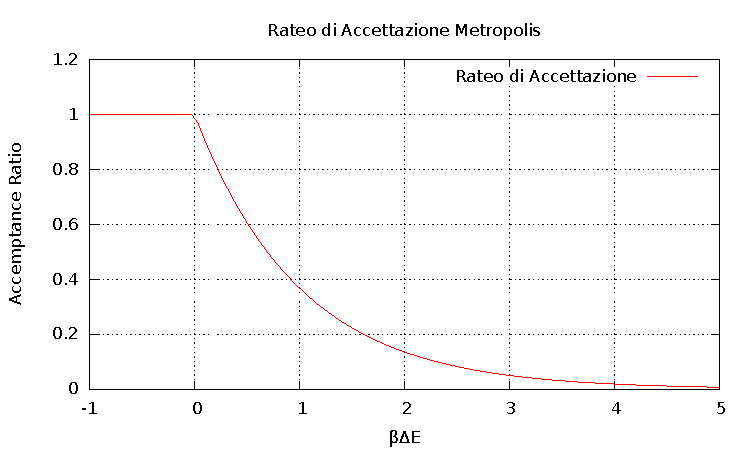
\includegraphics[width=120mm,angle=0,clip=]{acc_rat.pdf}
	\caption{Rateo di Accettazione Metropolis in funzione a $\beta \Delta E$}
	\label{acc_rat_met}
\end{figure}

Per il modello di Ising i \emph{ratei di accettazione} appena descritti hanno la particolarit\`a che possono essere calcolati mediante la sola conoscenza degli spins primi vicini allo spin di cui si propone il suo flip, questo perchè l'interazione nel modello di Ising  è a corto raggio. 

Nel caso dell'Hamiltoniana di Ising, questa differenza è possibile scriverla in modo molto semplice, in funzione solo dagli spin primi vicini dello spin di cui si propone il flip
\newl{
	E_\nu - E_\mu &=& -J\sum_{\langle i,j \rangle}s_i^\nu s_j^\nu + J\sum_{\langle i,j \rangle}s_i^\mu s_j^\mu = \nonumber\\
	&=& -J\sum_{i\neq k}s_i^\nu(s_k^\nu-s_k^\mu) = -2Js_k^\mu\sum_{i\neq k} s_i^\mu\,.
	\label{DIF:EN:SPIN}
}



\section{Implementazione del codice}
La strategia di implementazione che \`e stata adottata in questo lavoro consiste in una prima implementazione su CPU e la successiva implementazione su scheda grafica. L'obiettivo \`e quello di riottenere gli stessi risultati fisici e valutare lo \emph{speed-up} dato dall'utilizzo della GPU. 

La consistenza fisica della simulazione viene fatta comparando i grafici di \emph{Magnetizzazione} e \emph{Calore Specifico} in funzione di $\beta$, con la soluzione esatta di Onsager al limite Termodinamico. Successivamente sono stati confrontati gli stessi risultati ottenuti su GPU e CPU. 

Il secondo risultato che viene presentato riguarda le caratteristiche (punti favorevoli e punti sfavorevoli) di diversi PRNG, nel particolare \`e stato confrontato il numero di step di termalizzazione in funzione alla complessit\`a numerica della generazione. 

Il terzo risultato che viene presentato riguarda la ricerca di un BLOCKL di dimensione tale da portare a saturazione ogni singolo WARP. Tenendo in considerazione il fatto che in un blocco possono operare in modo parallelo $1024$ threads \`e necessario trovare il numero corretto di threads in $x$ e $y$ in modo da avvicinarsi il pi\`u possibile a $1024$.

Le conclusioni finali sull'ottimizzazione del programma terranno conto di tutte le conclusioni presentate precedentemente.

\section{Implementazione su CPU}
In Fig.~\ref{figura:CPU} sono presentati i risultati di \emph{Magnetizzazione} e \emph{Calore specifico}, per diversi size in funzione di $\beta$, comparati con la soluzione analitica al limite termodinamico di Onsager.

Si notano in modo evidente gli effetti di \emph{size-scaling} per reticoli molto piccoli. Al crescere della taglia del reticolo i risultati della simulazione si avvicinano sempre di pi\`u al modello al limite termodinamico.

I risultati riportati in Fig.~\ref{figura:CPU} mostrano anche che l'implementazione dell'algoritmo di update presentato nel capitolo precedente restituisce, su CPU, i valori attesi. Verificata la compatibilit\`a tra i valori numerici simulati e quelli teorici della soluzione di Onsager, \`e ora possibile passare all'implementazione su GPU con l'obiettivo di ottenere gli stessi risultati numerici valutando il relativo \emph{speed-up}.
\begin{figure}
	\centering
		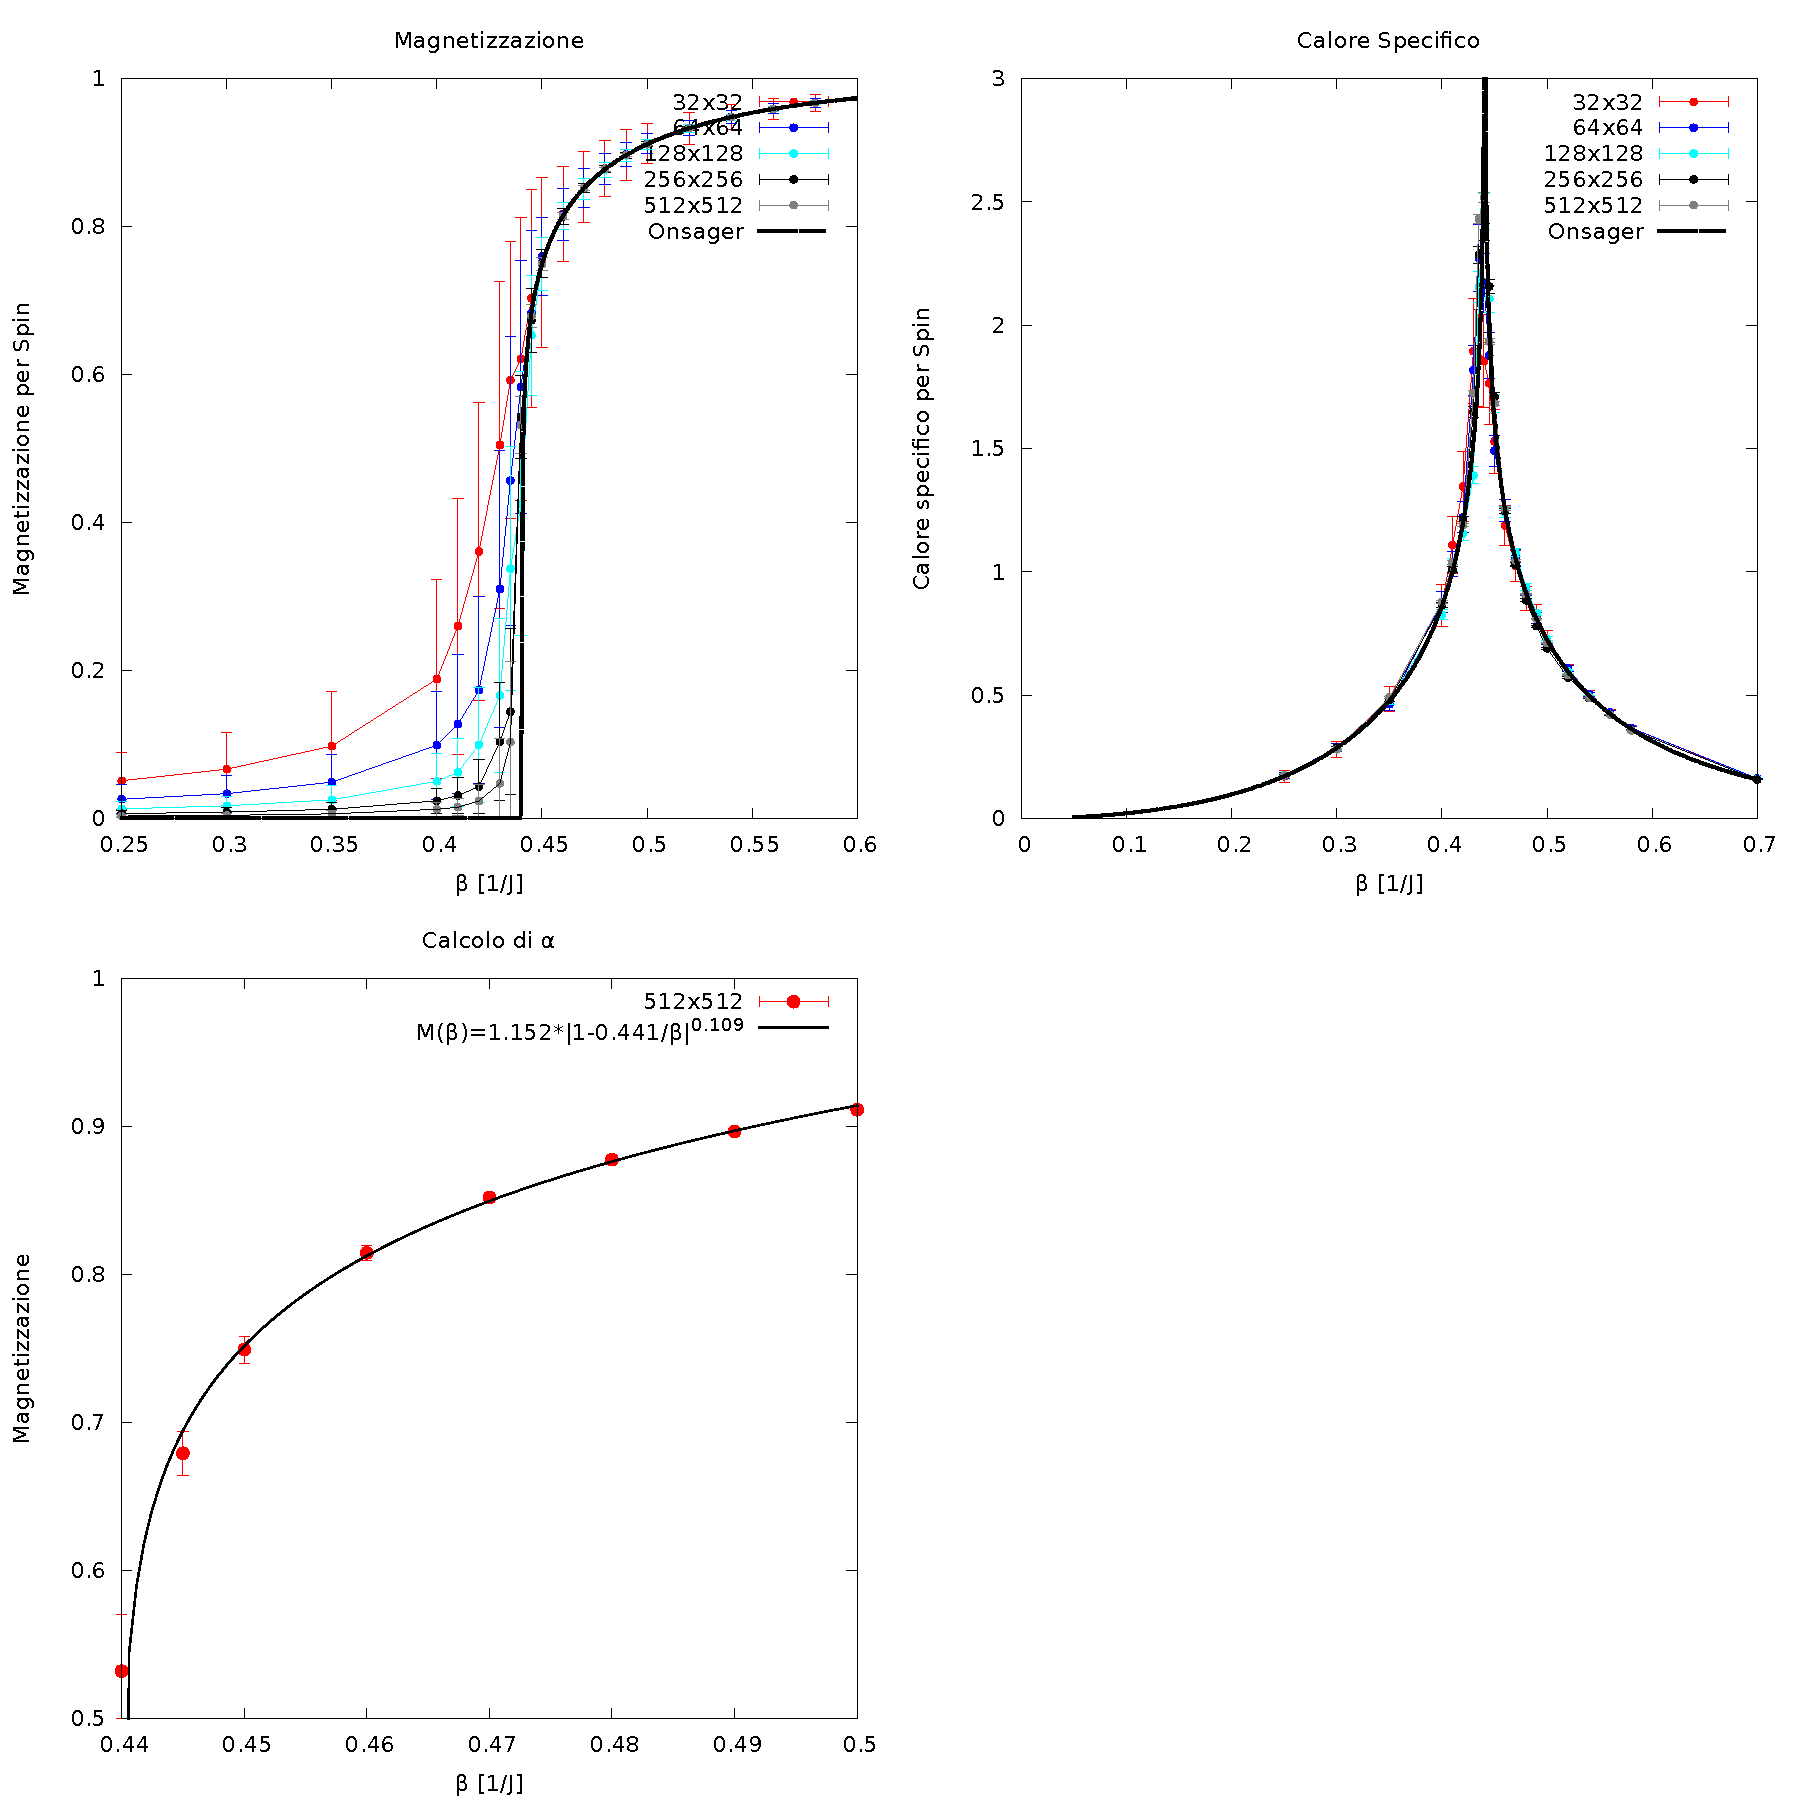
\includegraphics[width=120mm,angle=0,clip=]{../CPU/Result/Ising_Mag_Cv.pdf}
		\caption{\emph{Magnetizzazione} e \emph{Calore Specifico} per diverse taglie di reticolo, in funzione di $\beta$ generati su CPU}
		\label{figura:CPU}
\end{figure}

In Fig.~\ref{figura:randomCPU} viene presentato il confronto tra tre diversi PNRG. Come si nota, diversi generatori fanno termalizzare il sistema in un numero molto diverso di step. Tra i passi di termalizzazione del generatore pi\`u performante e quello meno performante c'\`e circa un fattore tre. 
\begin{figure}
\centering
	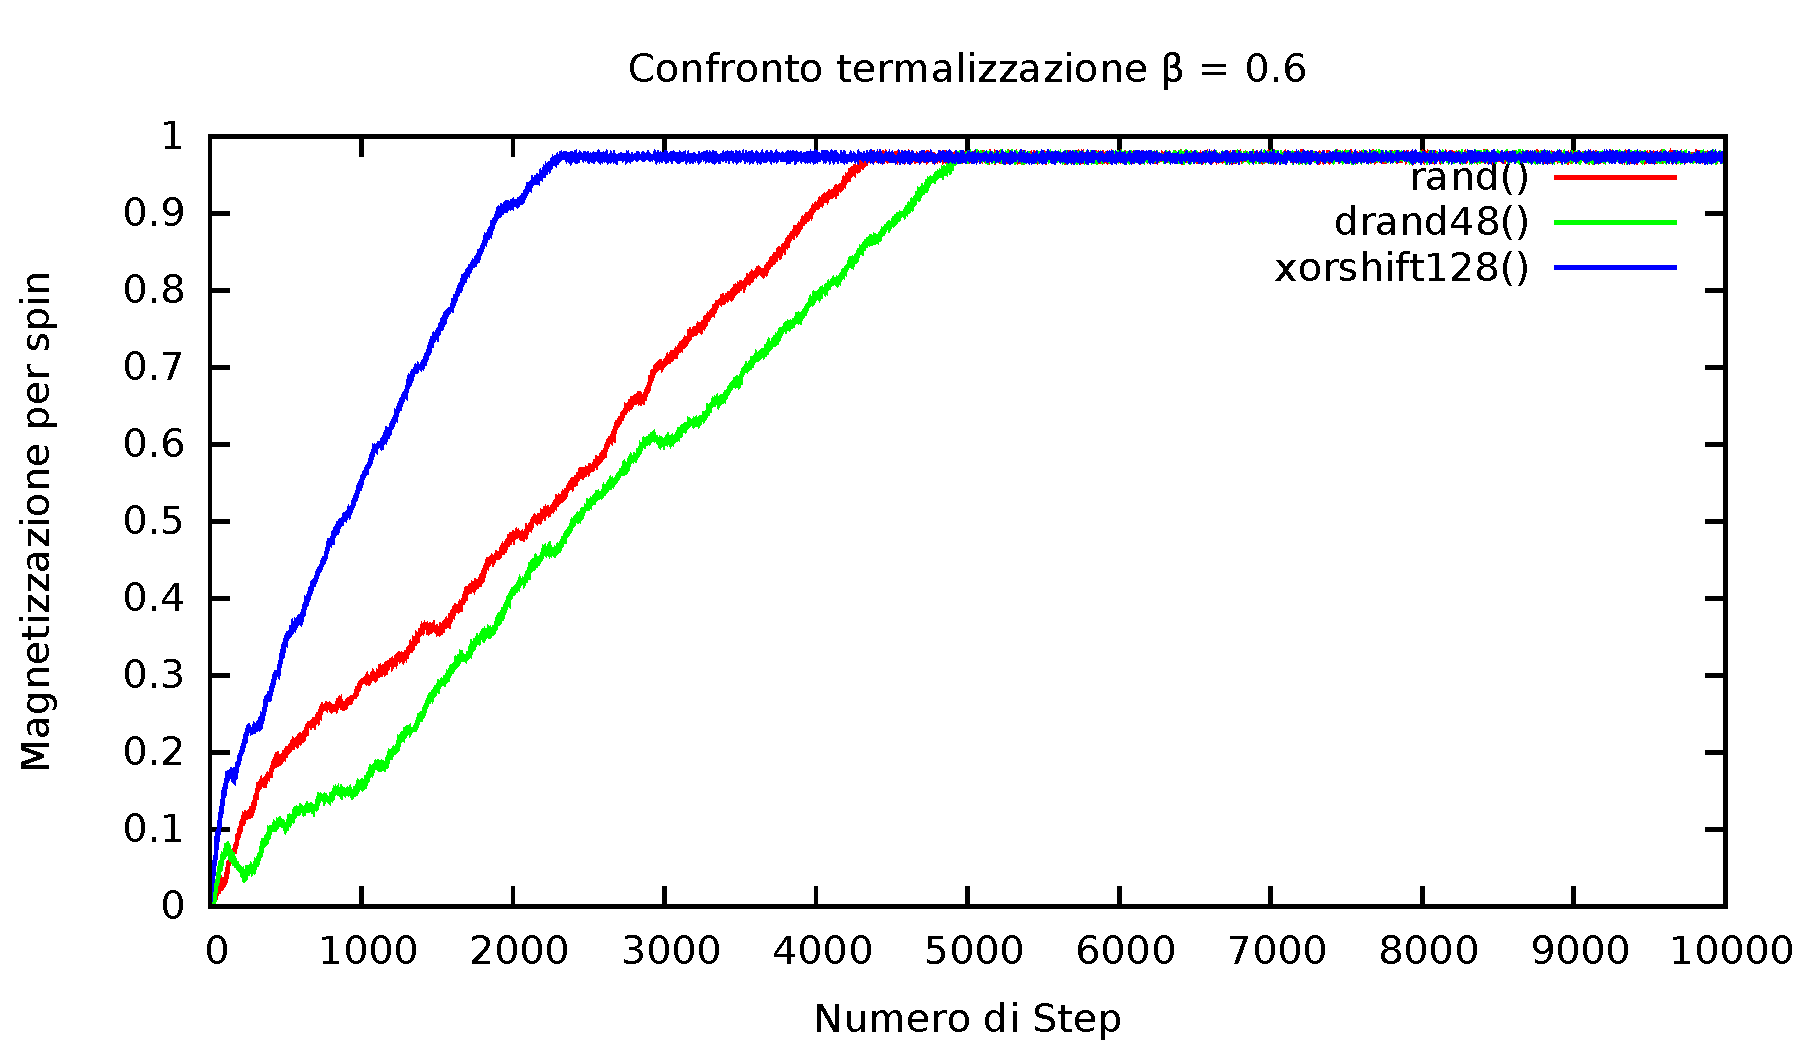
\includegraphics[width=120mm,angle=0,clip=]{../CPU/Result/Term_step.pdf}
	\caption{\emph{Passi Montecarlo} necessari per raggiungere la termalizzazione in funzione a tre diversi PNRG.}
	\label{figura:randomCPU}
\end{figure}
\section{Implementazione su GPU}
L'implementazione del codice su GPU \`e stata organizzata in modo da poter mettere in luce tutte le varie caratteristiche che contraddistinguono le \emph{schede grafiche}. La prima caratteristica \`e l'elevato numero di ALU\footnote{Arithmetic and Logic Unit} messo a disposizione rispetto alle CPU quindi una prima implementazione del codice \`e stata fatta portando il reticolo sulla \emph{memoria globale} della scheda e cercando di saturare il numero di ALU impegnate in modo parallelo attraverso una strategia di update a scacchiera.

La seconda caratteristica di questo tipo di devices \`e la possibilit\`a di ottimizzare il proprio programma usando tutti i vari \emph{livelli di memoria} che vengono messi a disposizione. Oltre alla \emph{memoria globale} \`e possibile usare un livello di memoria superiore chiamato \emph{memoria shared}. Il vantaggio di questo tipo di memoria consiste in una velocit\`a di lettura/scrittura superiore a quella globale. Lo svantaggio \`e che le sue dimensioni sono pi\`u piccole ed \`e suddivisa per blocco. Per far comunicare due dati, istanziati su blocchi diversi di memoria shared \`e necessario quindi scrivere delle condizioni di raccordo.

Un primo kernel naif che \`e possibile scrivere \`e quello che utilizza solo memoria globale e aggiorna gli spin seguendo solo una singola scacchiera. Un kernel pi\`u elaborato che sia in grado di gestire anche il livello di \emph{memoria shared} segue una strategia di update dei siti esposta in Fig.~\ref{reticolo_shared}.

Il kernel viene lanciato due volte con un parametro di offset. Al primo run vengono aggiornati tutti i blocchi rossi. A loro volta gli spin all'interno del blocco vengono aggiornati seguendo una strategia a scacchiera. \`E necessario organizzare anche una scacchiera tra i blocchi per non creare conflitto tra spin che rappresentano le condizioni di \emph{raccordo blocco-blocco}, che in Fig.~\ref{reticolo_shared} sono rappresentati dalla \emph{cornice gialla}.
\begin{figure}
	\begin{center}
		\begin{tikzpicture}[x=1.4cm,y=1.4cm]
		
		\foreach \p in {0,1,...,6}{
				\draw [ultra thick] (\p,0) -- (\p,6);
				\draw [ultra thick] (0,\p) -- (6,\p);
			}
		\foreach \p in {0,0.5,...,18}{
				\draw (\p/3,0) -- (\p/3,6);
				\draw (0,\p/3) -- (6,\p/3);
			}

		\foreach \blockx in {0,2,...,5}{
				\foreach \blocky in {0,2,...,5}{
					\fill [fill=red, opacity=0.5] (\blockx,\blocky) rectangle (\blockx+1,\blocky+1);
			}
		}
		\foreach \blockx in {0,2,...,5}{
				\foreach \blocky in {0,2,...,5}{
					\fill [fill=red, opacity=0.5] (\blockx+1,\blocky+1) rectangle (\blockx+2,\blocky+2);
			}
		}

		\fill [fill=yellow, opacity=0.7] (1,2) rectangle (2,2+0.5/3);
		\fill [fill=yellow, opacity=0.7] (1,1) rectangle (1-0.5/3,2);
		\fill [fill=yellow, opacity=0.7] (1,1) rectangle (2,1-0.5/3);
		\fill [fill=yellow, opacity=0.7] (2,1) rectangle (2+0.5/3,2);

		\foreach \a in {0,2,...,5}{
				\foreach \b in {0,2,...,5}{
					\fill [fill=black, opacity=0.7] (1+\a*0.5/3,1+\b*0.5/3) rectangle (1+\a*0.5/3+0.5/3,1+\b*0.5/3+0.5/3);
			}
	}
		\foreach \a in {0,2,...,5}{
				\foreach \b in {0,2,...,5}{
					\fill [fill=black, opacity=0.7] (1+\a*0.5/3+0.5/3,1+\b*0.5/3+0.5/3) rectangle (1+\a*0.5/3+2*0.5/3,1+\b*0.5/3+2*0.5/3);
			}
	}

		\end{tikzpicture}
	\end{center}
	\caption{Strategia di update a doppia scacchiera. I blocchi vengono attivati a scacchiera. In ogni blocco, l'update degli spin \`e a sua volta fatto a scacchiera. In giallo sono identificati gli spin di \emph{cornice} che devono essere storati nella memoria shared, di ogni blocco, per garantire la condizione di raccordo \emph{blocco-blocco} }
	\label{reticolo_shared}
\end{figure}


\subsection{Consistenza del modello Fisico su GPU}
In Fig.~\ref{figura:CPU} e Fig.~\ref{figura:GPU} vengono rappresentati tre grafici per ogni immagine. Il primo rappresenta la magnetizzazione (per spin) in funzione di $\beta$, il secondo il calore specifico per spin sempre in funzione di $\beta$ e nel terzo viene fatto un fit dei valori di magnetizzazione, per ricavare l'esponente critico $\alpha$. 

Nell'intorno del $\beta_c$ la magnetizzazione si comporta come
\newl{M(\beta)\sim \left\lvert 1-\frac{\beta_c}{\beta}\right\rvert ^{\alpha}.}
Effettuando un fit dei valori intorno alla temperatura critica, lasciando come parametri liberi $\alpha$ e $\beta_c$ è quindi possibile ricavare il valore dell'esponente critico e della temperatura critica di transizione di fase. In Fig.~\ref{figura:CPU} e Fig.~\ref{figura:GPU} sono riportati i valori del fit trovati che sono compatibili con quelli noti.

\begin{figure}
	\centering
		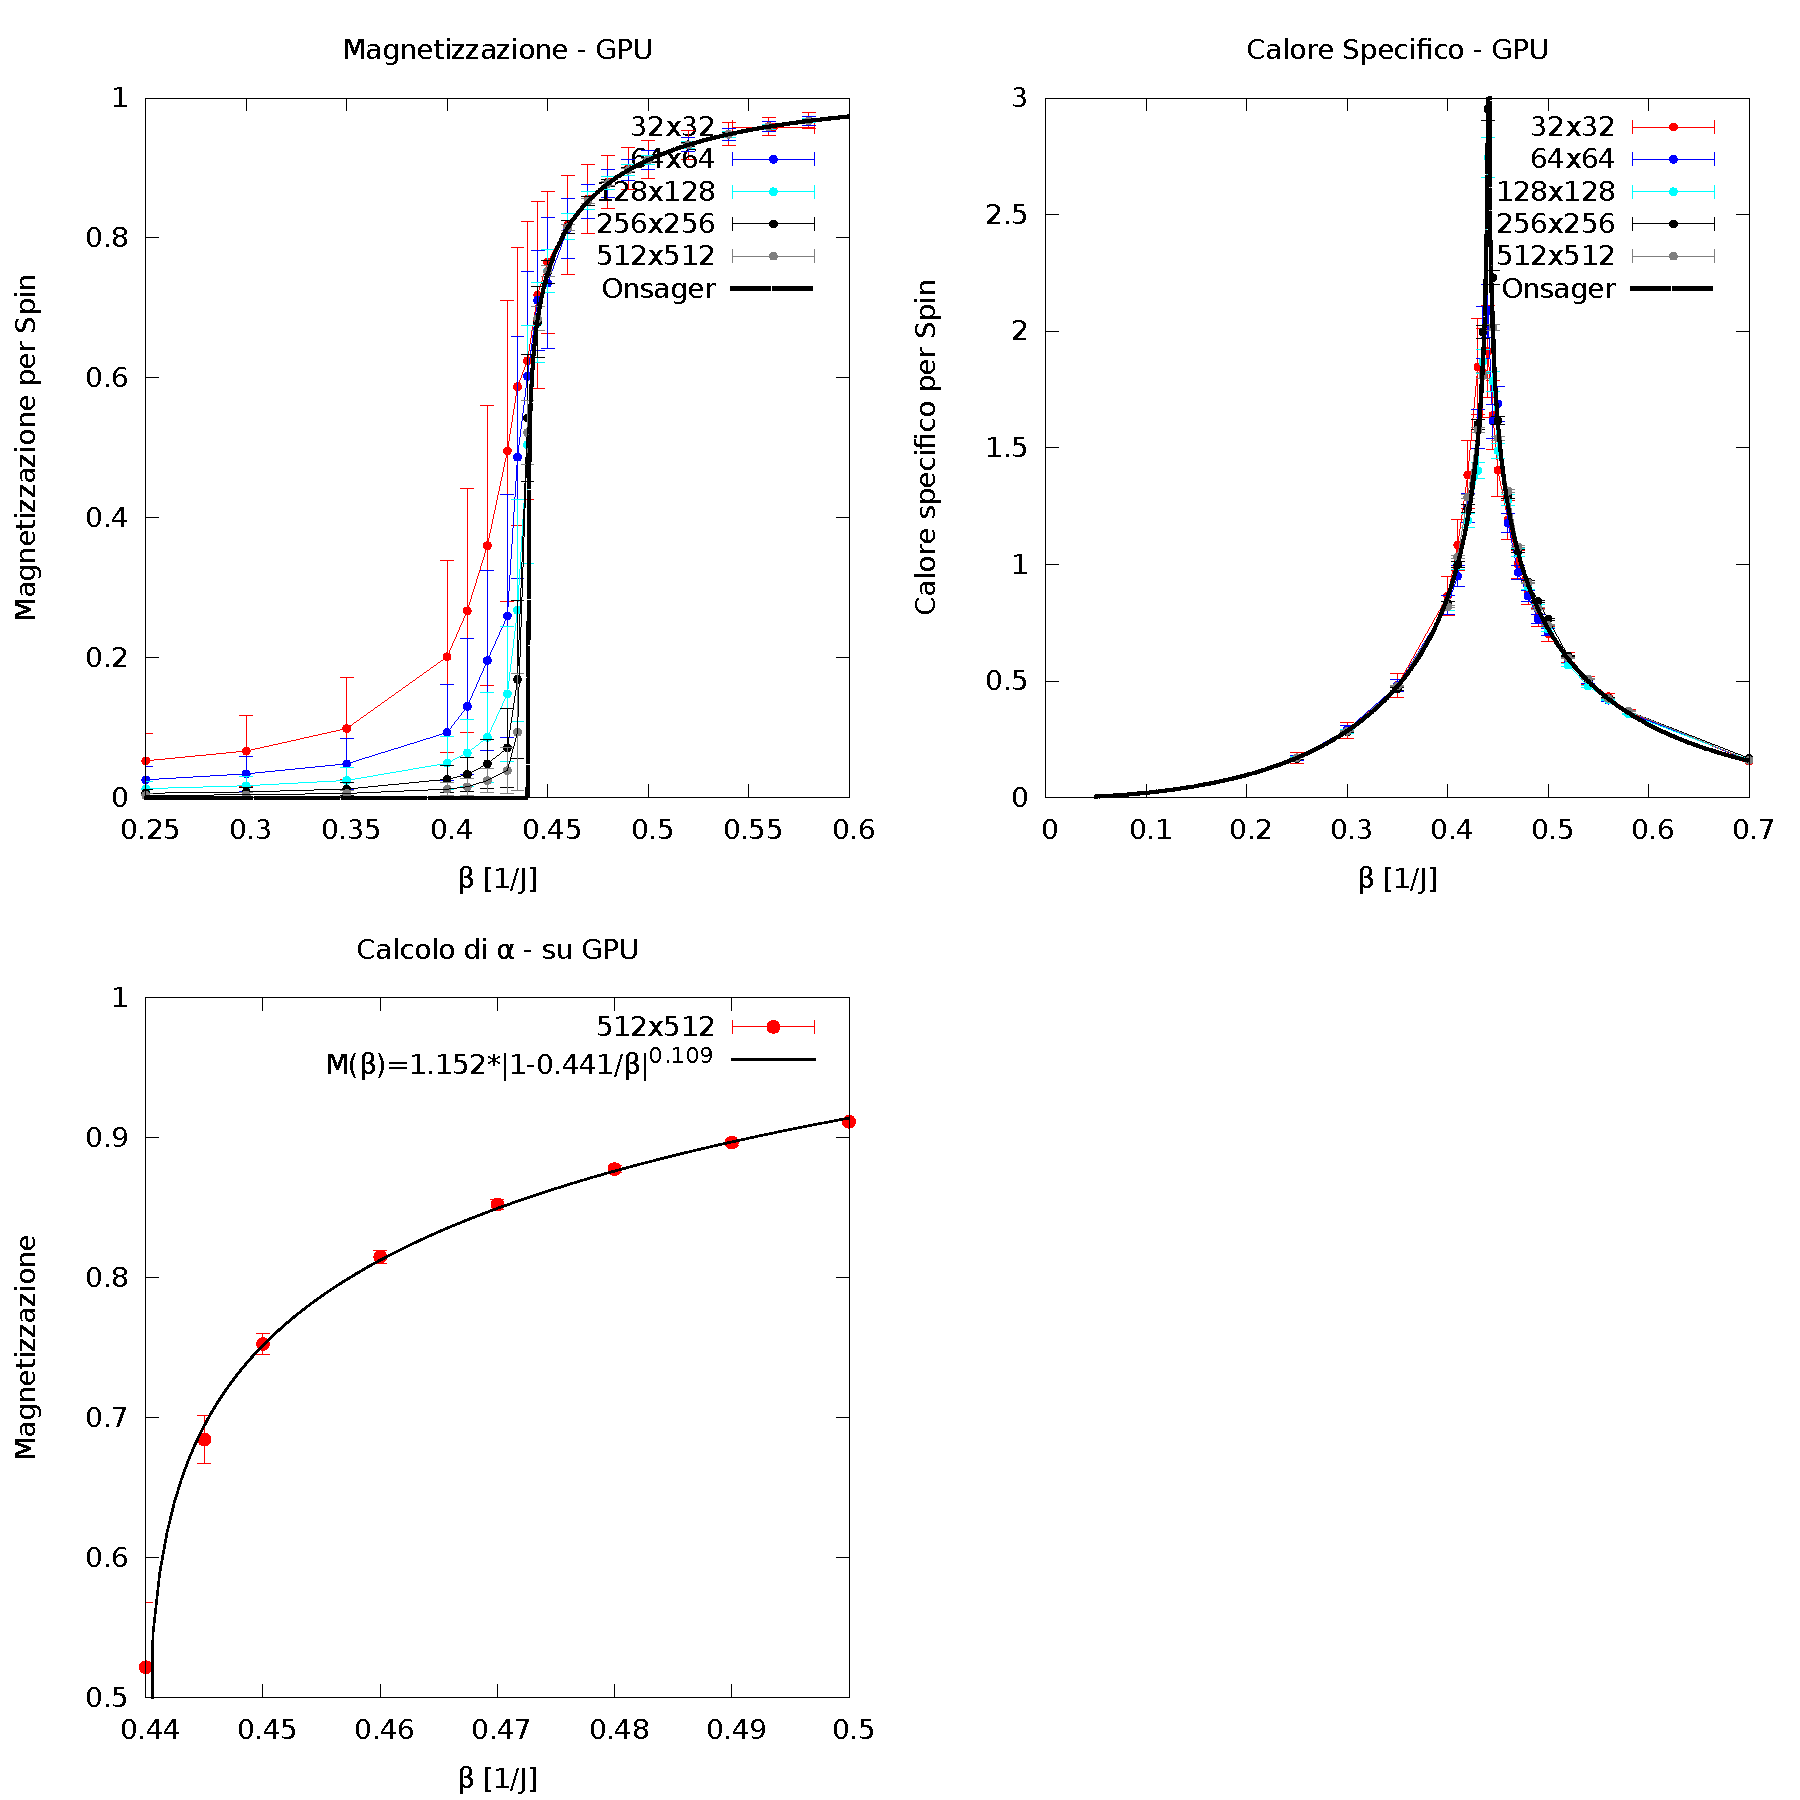
\includegraphics[width=120mm,angle=0,clip=]{../CUDA/Result/Res3/Ising_Mag_Cv.pdf}
		\caption{\emph{Magnetizzazione} e \emph{Calore Specifico} per diverse taglie di reticolo, in funzione di $\beta$ generati su GPU}
		\label{figura:GPU}
\end{figure}

\subsection{Confronto performance dei vari PNRG}
Insieme al numero di step necessari a far termalizzare il sistema \`e necessario indagare anche le performance temporali di ogni singolo PNRG per verificare se l'effettivo guadagno in numero di step \`e un effettivo guadagno in termini di tempi di simulazione. 

Un generatore caratterizzato da una miglior statistica e randomicit\`a dei dati pu\`o far termalizzare prima il sistema ma va comunque valutato il costo temporale necessario a generarli.
\begin{figure}
	\centering
		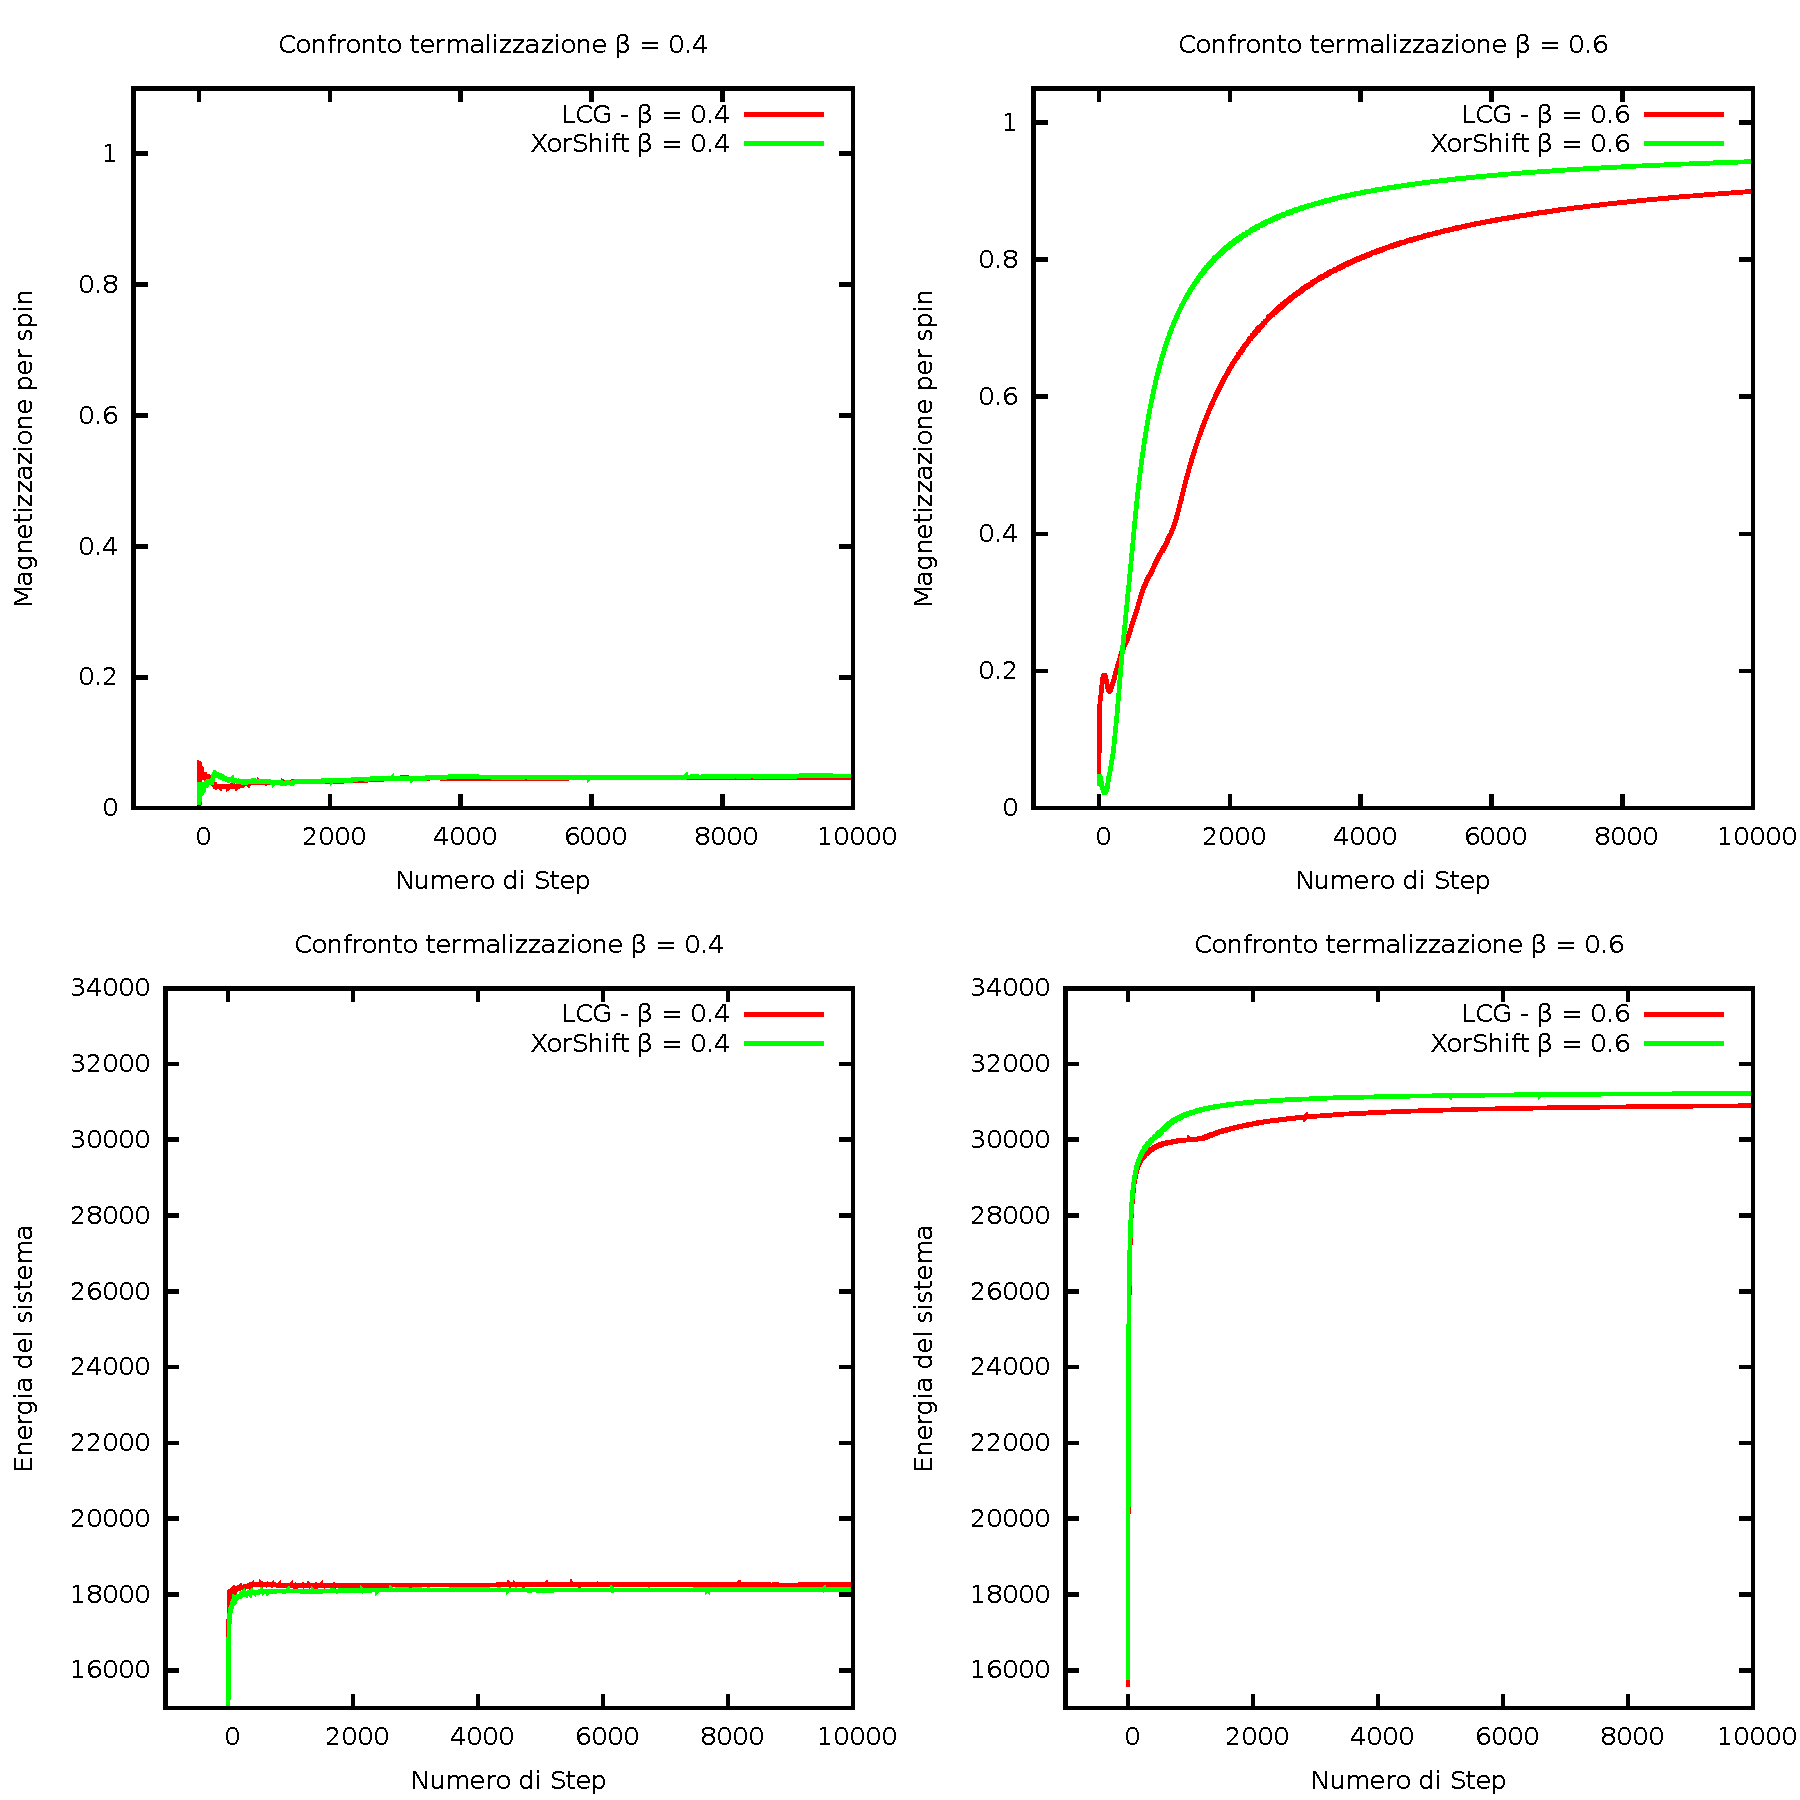
\includegraphics[width=120mm,angle=0,clip=]{../CUDA/Term/Term_step_GPU_04.pdf}
		\caption{Termalizzazione per due differenti PNRG. In rosso LCG a 32 bit, in verde XorShift a 128 bit per un reticolo \emph{128$\times$128} spins}
		\label{termalizz:GPU}
\end{figure}
\begin{figure}
	\centering
		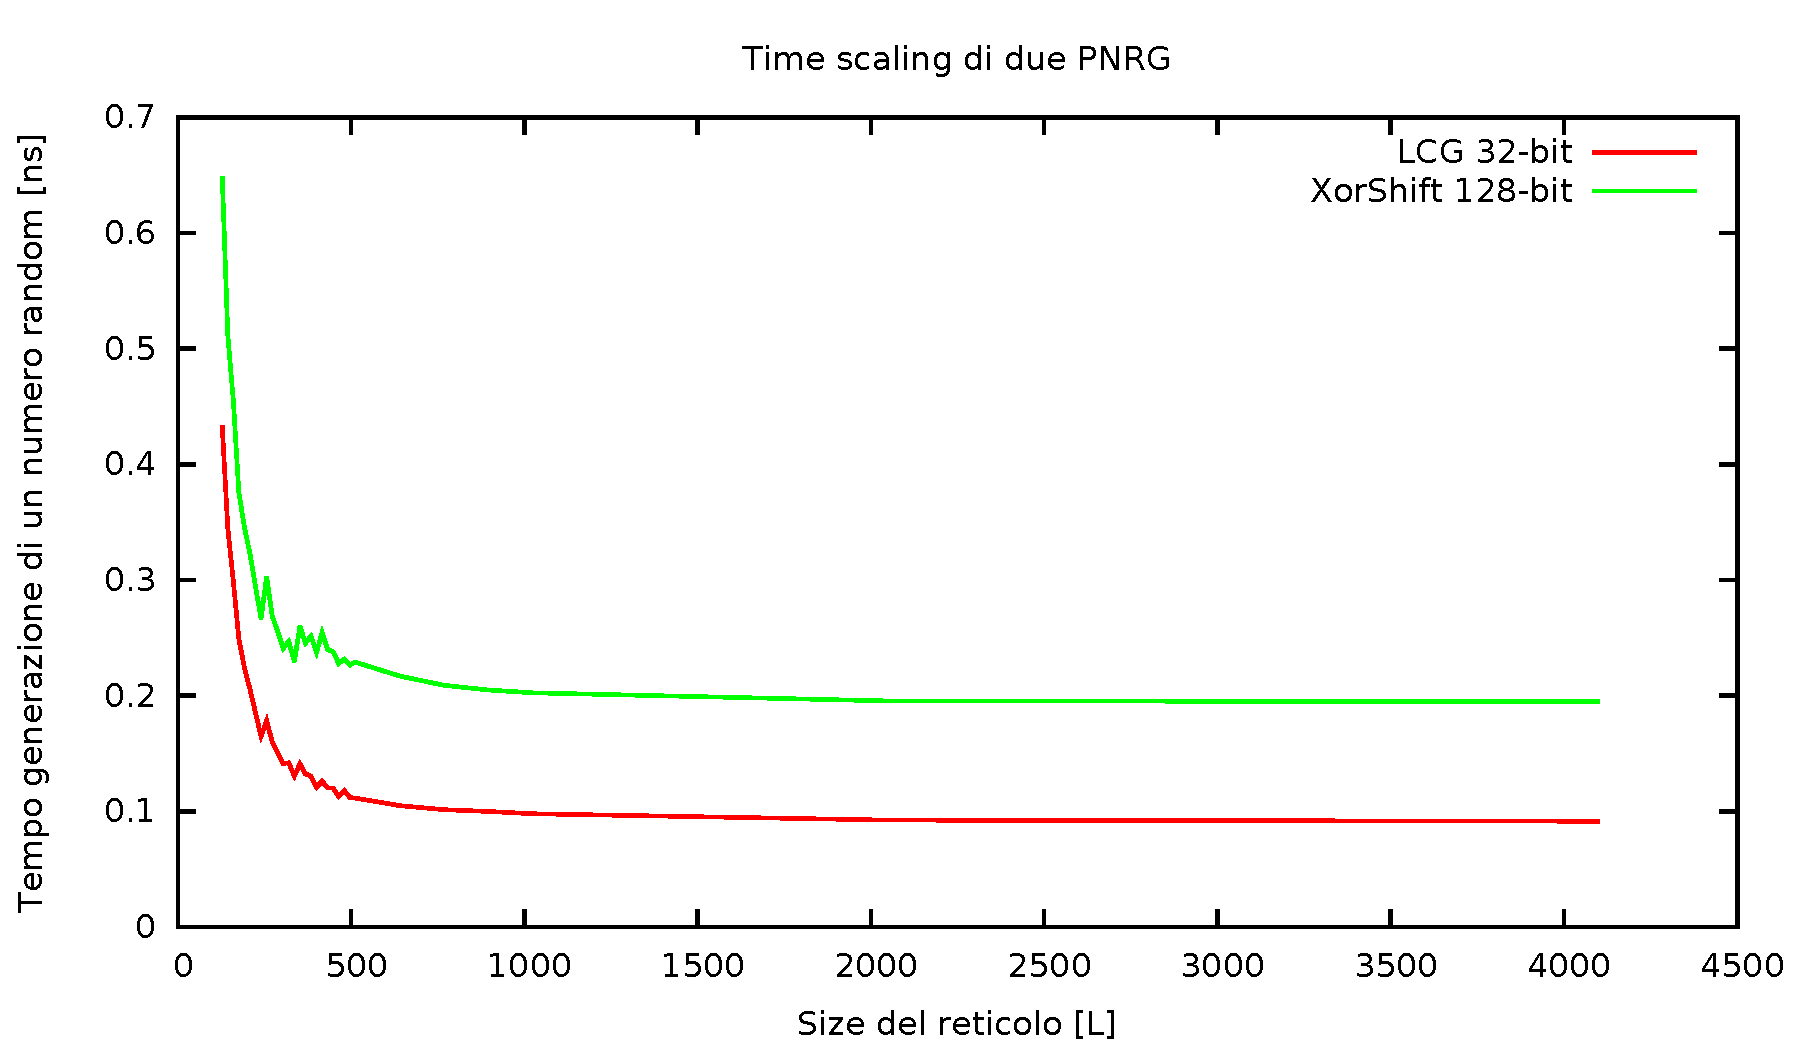
\includegraphics[width=120mm,angle=0,clip=]{../CUDA/Result/Res3/Time_PNRG.pdf}
		\caption{Confronto del tempo di generazione di un numero pseudorandom per due differenti PNRG}
		\label{time:per:random}
\end{figure}
Mettendo insieme i risultati esposti in Fig.~\ref{termalizz:GPU} ed in Fig.~\ref{time:per:random} si pu\`o notare che, il numero di step necessari alla termalizzaione \`e legato in qualche modo a $\beta$. Per valori di $\beta$ piccoli (inferiori a $\beta_c$) i due PNRG fanno termalizzare il sistema nello stesso modo. Diminuendo la temperatura a $\beta=0.6$, ci si va a posizionare nella zona a decadimento esponenziale del rateo di accettazione che \`e stato presentato in Fig.~\ref{acc_rat_met}. Dato che una mossa viene accettata solo se il numero random estratto si va a posizionare sotto alla curca del rateo di accettazione, nella parte piccola diventa pi\`u eviente la qualit\`a dei numeri pseudorandom che vengono generati.

A bassa temperatura l'algorimo \emph{XorShift 128-bit} impiega circa $1600$ step a termalizzare. Con la funzione \emph{rand 31-bit} impega quasi $4000$ step, quindi un generatore a $31bit$ impega circa $2.5$ volte in pi\`u a termalizzare rispetto ad uno a $128$ bit. Per quanto riguardo i tempi, un generatore a $128-bit$, rispetto ad uno a $32-bit$ \`e solamente $2$ volte pi\`u lento. Questo fa s\`i che la soluzione pi\`u performante, per $\beta>\beta_c$, sia quella che prevede di utilizzare un generatore di numeri pseudorandom pi\`u lento ma che permetta al sistema di termalizzare in un numero inferiori di step Monte Carlo. Per $\beta < \beta_c$ risulta pi\`u performanete l'algoritmo a $32-bit$.

\subsection{Compatibilit\`a statistica dei risultati}
In Tab.~\ref{tab:mag} sono riportati i valori di magnetizzazione per un reticolo $32\times32$, con relativo errore, in funzione di $\beta$. Come detto in precedenza si è riusciti a riportare completamente, operazione per operazione, l'algoritmo usato su CPU alle schede grafiche quindi ci si aspetta che dopo lo stesso numero di passi Monte Carlo, il dato sia proprio identicamente lo stesso. 

Come si può notare in Tab.~\ref{tab:mag} i dati, seppur compatibili tra loro all'interno del proprio errore, non sono identicamente lo stesso dato. La spiegazione consiste nel modo in cui vengono estratti i numeri pseudocasuali. Nel caso dell CPU l'evoluzione di uno spin è caratterizzato da un certo numero PR della catena e così via in modo ordinato su tutta l'estensione del reticolo, per tutti gli step Monte Carlo usati. 

Nel caso della GPU, la catena di numeri pseudo random viene suddivisa in sottocatene. Il numero pseudorandom che caratterizava l'evoluzione dello spin nominato precedentemente, sulla GPU può caratterizzare un altro spin. \`E  quindi corretto trovare valori differenti, ma compatibili entro il loro errore statistico. 

In conclusione i dati ci indicano che nonostante ci sia un rimescolamento dei numeri casuali, la statistica del sistema rimane sempre la stessa quindi le due simulzioni su CPU e GPU restituiscono risultati compatibili tra loro. Entrambi i risultati hanno un andamento compatibile con quello atteso se confrontati col modello al limite termodinamico.   

\begin{table}
\begin{center}
\begin {tabular}{c|c|c|c|c}
\hline
\hline
$\beta$ & $\langle  M \rangle$-GPU & $\sigma_{\langle  M \rangle-GPU}$ & $\langle  M \rangle$-CPU & $\sigma_{\langle  M \rangle-CPU}$        \\
\hline
$0,250000$ &    $0,052712$   &     $0,039474$ &  $0,050932$  &  $0,038267$\\
$0,300000$ &     $0,066671$     &   $0,050460$ &  $0,066645$  &  $0,049545$\\
$0,350000$ &      $0,098850$    &    $0,072529$ &  $0,097678$  &  $0,073882$\\
$0,400000$ &      $0,201638$   &     $0,137473$  &  $0,188406$  &  $0,134147$\\
$0,410000$ &       $0,267280$   &     $0,174247$  &  $0,260063$  &  $0,172984$\\
$0,420000$ &       $0,360316$   &     $0,199749$  &  $0,360821$  &  $0,201873$\\
$0,430000$ &       $0,495578$   &     $0,214933$  &  $0,504824$  &  $0,220384$\\
$0,435000$ &       $0,587416$   &     $0,199017$  &  $0,592545$  &  $0,186706$\\
$0,440000$ &       $0,624490$   &     $0,198886$  &  $0,621196$  &  $0,190946$\\
$0,445000$ &       $0,718453$   &     $0,133490$  &  $0,703127$  &  $0,147649$\\
$0,450000$ &       $0,765466$   &     $0,101283$  &  $0,751676$  &  $0,115272$\\
$0,460000$ &       $0,818402$   &     $0,070646$  &  $0,817304$  &  $0,063977$\\
$0,470000$ &       $0,855991$   &     $0,049240$  &  $0,853003$  &  $0,048010$\\
$0,480000$ &       $0,880319$   &     $0,037618$  &  $0,878726$  &  $0,038106$\\
$0,490000$ &       $0,899063$   &     $0,030522$  &  $0,896382$  &  $0,034484$\\
$0,500000$ &       $0,912002$   &     $0,026942$  &  $0,912000$  &  $0,027388$\\
$0,520000$ &       $0,933304$   &     $0,020621$  &  $0,932910$  &  $0,021438$\\
$0,540000$ &       $0,948533$   &     $0,016265$  &  $0,948100$  &  $0,016604$\\
$0,560000$ &       $0,959347$   &     $0,013461$  &  $0,958931$  &  $0,013762$\\
$0,580000$ &       $0,967683$   &     $0,011340$  &  $0,967213$  &  $0,011583$\\
$0,700000$ &       $0,990200$   &     $0,005175$  &  $0,990184$  &  $0,005217$\\
\\
\hline
\hline
\end{tabular}
\end{center}
\caption{\label{tab:mag}
	Valori di magnetizzazione con il loro errore.
}
\end{table}

\subsection{Ottimizzazione della dimensione del blocco}
La dimensione del numero di threads appartenenti ad un blocco \`e un parametro che pu\`o essere scelto nel programma. In Fig.~\ref{time:block:size} viene presentato l'andamento del tempo di run in funzione della dimensione del blocco.

Come \`e possibile notare, il minimo \`e facilmente identificabile a $BLOCKL=24$. Questo valore trova la sua spiegazione in come \`e costruita la scheda grafica. Per la GTX480, il numero di threads che possono essere contenuti in un blocco \`e al massimo $1024$\footnote{Dato ottenuto con cudaGetDeviceProprieties()}.

La spiegazione di questo risultato \`e nelle modalit\`a di lancio del kernel. Per effettuare la doppia scacchiera viene passata una $dimBlock$  sotto forma di struttura $dim3$ in cui il numero di threads in Y \`e la met\`a di quelli in X. Chiamando $BLOCKL$ la dimensione del blocco in Y, risulta che in un blocco, per ogni lancio del kernel ci sono un numero di threads che \`e pari a $2*BLOCKL*BLOCKL$. Il valore di $BLOCKL$ che permette a questa espressione di saturare completamente il warp \`e appunto $24$ in quanto $24*24*2=1152$. Quindi, per ottenere le migliori performance \`e opportuno scegliere una dimensione del blocco in modo da permettere la saturazione del Warp.
\begin{figure}
	\centering
		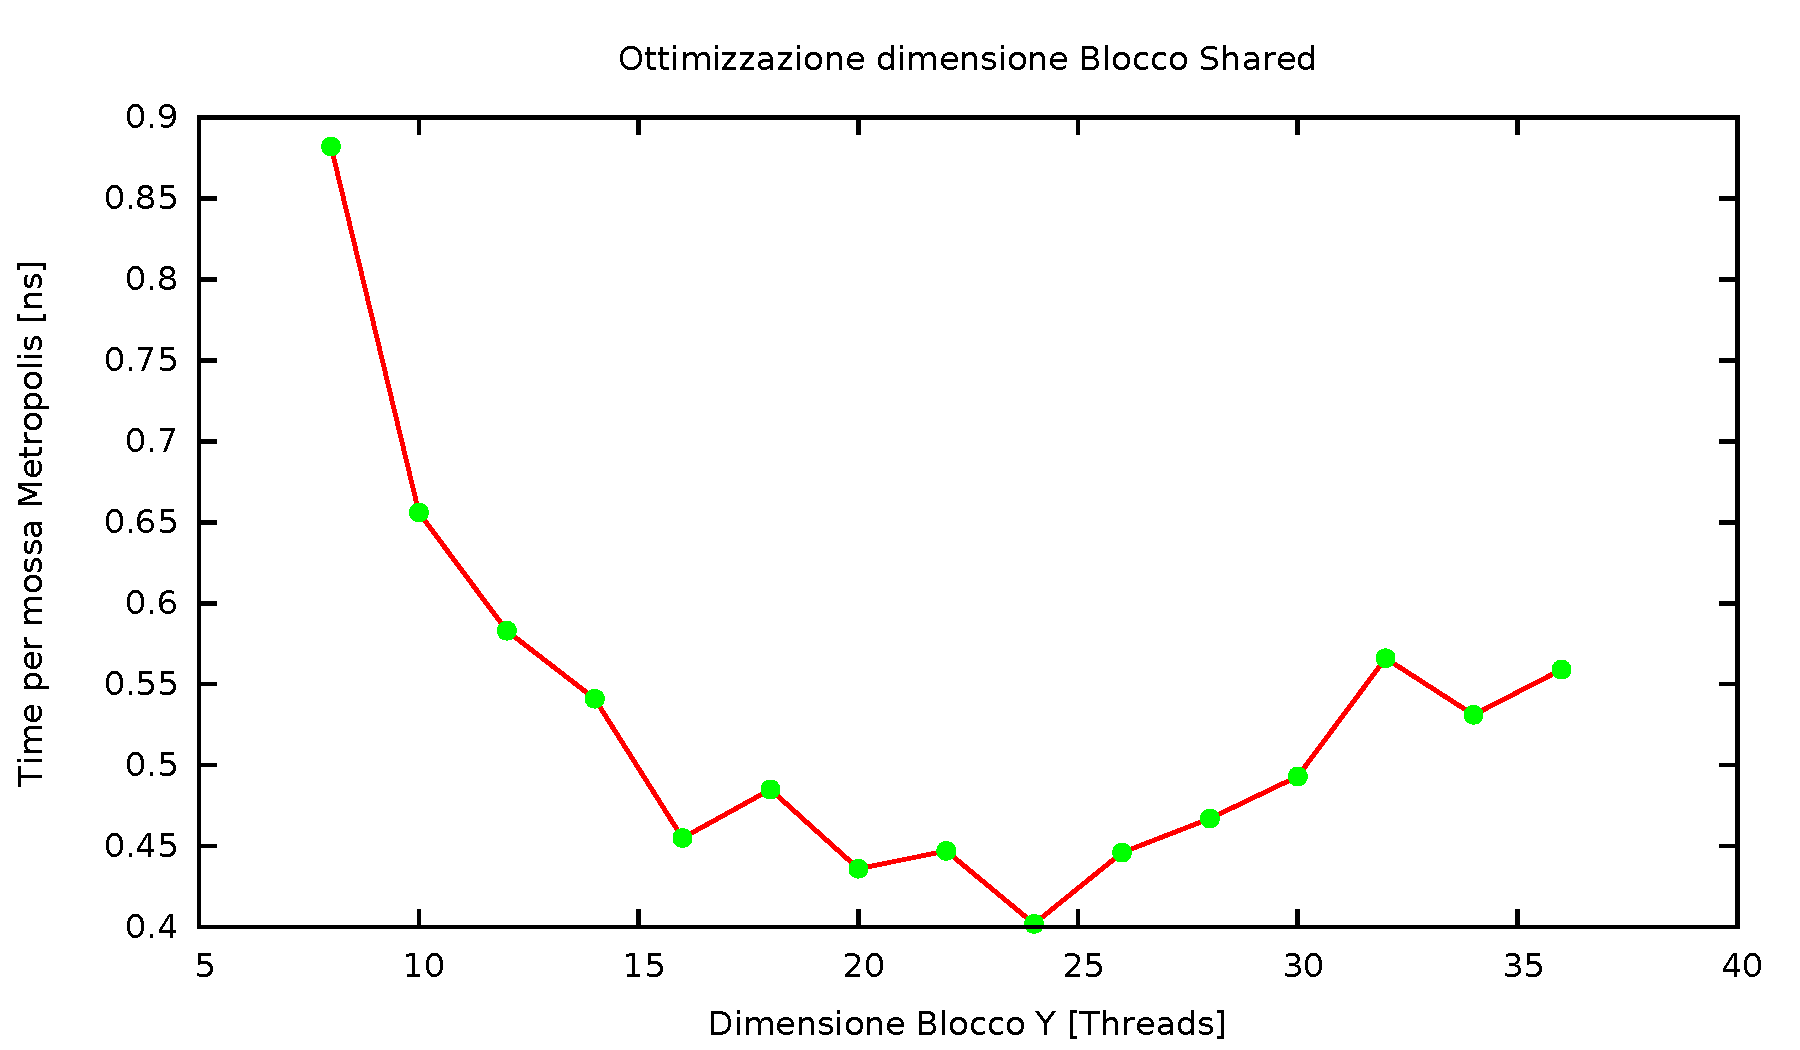
\includegraphics[width=120mm,angle=0,clip=]{../CUDA/Result/Res3/Time_BLOCK.pdf}
		\caption{Tempo di esecuzione in funzione alla dimensione del Blocco}
		\label{time:block:size}
\end{figure}


\section{Comparazione delle prestazioni}
Il codice è stato implementato in CPP per singola CPU, ed in cuda C con due varianti, la prima con il reticolo tutto su global memory la seconda utilizzando anche la memoria shared. I risultati sono riportati in Figura \ref{figura:time}. 

Come è possibile notare, una volta saturato il sensore, lo speed-up raggiunto è nell'ordine dei $2$ ordini di grandezza rispetto allo stesso codice girato du CPU. 

L'utilizzo della memoria shared porta vantaggi solo per reticolo molto grandi. Questo era attendibile in quanto, essendo il modello di Ising molto semplice da implementare, il fatto di avere tutto il reticolo su memoria globale d\`a particolari problemi dal punto di vista della coalescenza della memoria. Per reticoli piccoli, infatti, il guadagno che si ha in lettura/scrittura lo si perde tutto nella complessit\`a di posizionare il reticolo nei blocchi di memoria shared e nell'imporre le condizioni di raccordo tra i blocchi.
Per reticoli molto grossi il guadagno in termini di lettura/scrittura diventa pi\`u incisivo. Essendo moltissimi spin, diventano molto incisive le operazioni di lettura e scrittura. Quello che prima veniva perso nella complessit\`a delle condizioni di raccordo ora \`e poco incisivo rispetto al numero di letture/scritture.
\begin{figure}
	\centering
	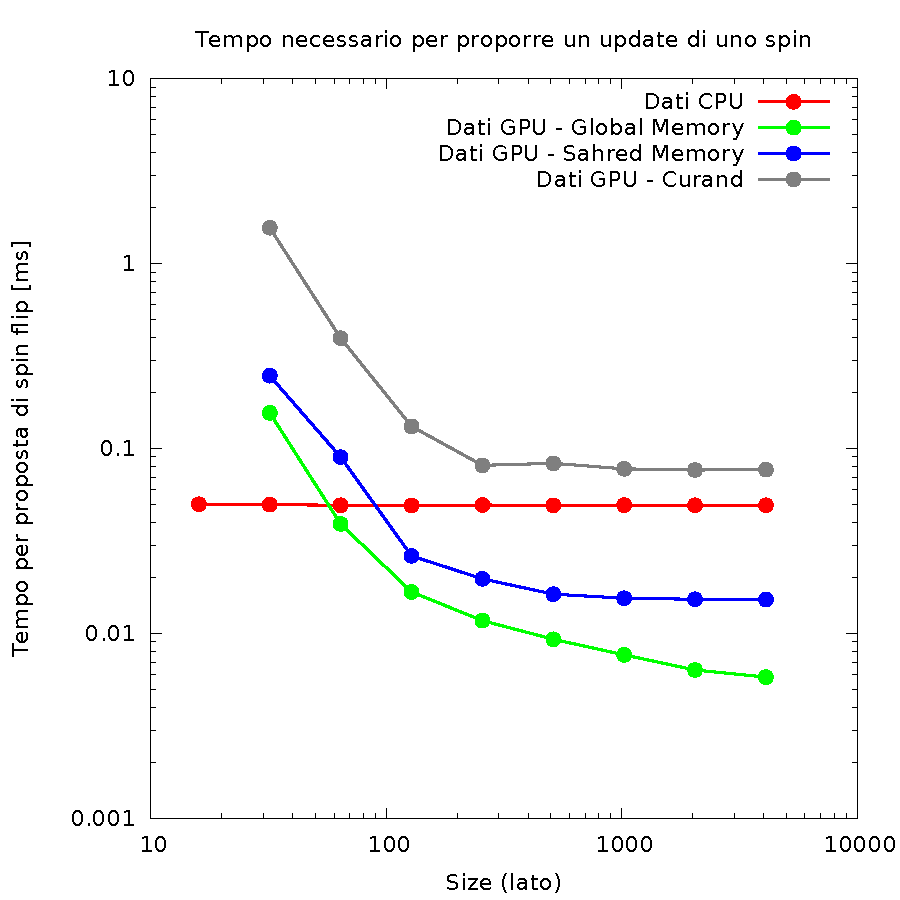
\includegraphics[width=150mm,angle=0,clip=]{../CPU-GPU-time.pdf}
	\caption{Confronti tempi di esecuzione per CPU, GPU global memory e GPU shared memory}
	\label{figura:time}
\end{figure}


\end{document}
